
%%%%%%%%%%%%%%%%%%%%%%% file typeinst.tex %%%%%%%%%%%%%%%%%%%%%%%%%
%
% This is the LaTeX source for the instructions to authors using
% the LaTeX document class 'llncs.cls' for contributions to 
% the Lecture Notes in Computer Sciences series.
% http://www.springer.com/lncs       Springer Heidelberg 2006/05/04
%
% It may be used as a template for your own input - copy it 
% to a new file with a new name and use it as the basis
% for your article. 
%
%%%%%%%%%%%%%%%%%%%%%%%%%%%%%%%%%%%%%%%%%%%%%%%%%%%%%%%%%%%%%%%%%%%


%\documentclass[runningheads]{llncs}
\documentclass{llncs}
%\documentclass{article}

%\usepackage[active]{srcltx}
\usepackage{amssymb}
\usepackage{array}
\setcounter{tocdepth}{3}
\usepackage{graphicx}
\usepackage{listings}

\usepackage{natbib}
\bibpunct{(}{)}{;}{a}{}{,}

%\usepackage{url}
%\urldef{\mailsa}\path|{Daniel.Marbach, Claudio.Mattiussi, Dario.Floreano}@epfl.ch|
\newcommand{\keywords}[1]{\par\addvspace\baselineskip
\noindent\keywordname\enspace\ignorespaces#1}

\newcommand{\insilico}{\emph{in silico }}
\newcommand{\invivo}{\emph{in vivo }}
% \newcommand{\gnw}{{\neuropol{GNW}} }

%\font\neuropol=neuropol
%\font\neuropolLarge=neuropol at 36pt
% \setlength{\parskip}{6pt plus3pt minus2pt}
% \baselineskip=8pt
% \addtolength{\parskip}{\baselineskip}
\parindent 0ex



\newenvironment{mylist}{
\begin{itemize}
%   \setlength{\itemsep}{0pt}
%   \setlength{\parsep}{0pt}
%   \setlength{\parskip}{6pt plus3pt minus2pt}
}{\end{itemize}}

\newenvironment{myenum}{
\begin{enumerate}
%   \setlength{\itemsep}{6pt plus3pt minus2pt}
%   \setlength{\parskip}{0pt}
%   \setlength{\parsep}{0pt}
}{\end{enumerate}}

\begin{document}

% \pagestyle{plain}
% \sffamily

\begin{center}

% \center \Huge GNW User Guide
\center %\neuropolLarge{GNW} 
GNW \Huge User Guide

\vspace{0.5cm}

\Large 
GeneNetWeaver Version 1.2

\vspace{0.5cm}

Thomas Schaffter \& Daniel Marbach

firstname.name@gmail.com

\vspace{0.5cm}

February 16, 2009

\vspace{0.5cm}

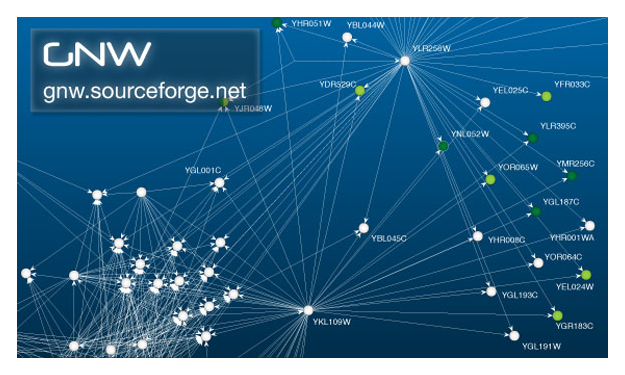
\includegraphics[width=10cm]{figures/user-guide-title}

\vspace{0.8cm}

Ecole Polytechnique F\'ed\'erale de Lausanne (EPFL),\\
Laboratory of Intelligent Systems,\\
CH-1015 Lausanne, Switzerland

\vspace{0.5cm}

http://lis.epfl.ch/grn\\
http://gnw.sourceforge.net

\end{center}

\vspace{\stretch{1}}

\pagebreak

\tableofcontents

\vspace{\stretch{1}}
\pagebreak

% ==================================================================================

\section{Introduction}
\textbf{Important}: Before you start, you may want to read our website (gnw.sf.net) for a short introduction to GNW and the science behind it.

\subsection{Overview}

GeneNetWeaver (GNW) is a tool for the automatic generation of \emph{in silico}\footnote{With ``\emph{in silico}'' we mean in simulation, as opposed to \emph{in vivo}, which would be in the real biological cell.} gene networks and reverse engineering benchmarks. GNW was used to generate the \textit{DREAM3 In Silico Challenges}, which are currently the most widely used gene network reverse engineering benchmark in the community.\\

You can launch GNW directly from your browser by clicking the \emph{Launch GNW} button on the top right of our website (gnw.sf.net). If it doesn't work, make sure that you have Java Web Start installed.

\subsection{License / how to cite us}

GNW is released open-source under an MIT license. If you use GNW for your research, please cite \citet{Marbach2009}.

\subsection{Using this manual}

The purpose of this manual is to explain the different functionalities offered by GNW. The algorithms and models that GNW is based upon are not explained here. If you intend to use GNW for your research, we recommend first reading our publications listed in the bibliography.

\subsection{How to contact the GNW project}

The GNW project can be contacted via its website (gnw.sf.net). Please feel free to contact us with bug reports, feature requests, and information on related projects.

\vspace{\stretch{1}}
\pagebreak

% ==================================================================================

\section{Getting Started}

\subsection{Launching GNW}

GNW is ditributed through the Java Web Start technology developed by Sun. This allows any computer on which Java Web Start is installed to run GNW, independently of the operating system used. GNW requires Java version 1.5 or later.\\

Launching GNW is as simple as one click! Please visit the project website (gnw.sf.net) from where you will be able to run GNW by clicking on the \emph{Launch GNW} button. If it doesn't work, make sure that you have Java Web Start installed\footnote{http://java.sun.com/products/javawebstart}. Java Web Start will download the application and ask whether you trust the \emph{LIS Certificate}. You must accept the certificate in order to run GNW.

\begin{figure}[h!]
\centering
\includegraphics[width=10cm]{figures/certificate}
\caption{Click \emph{Trust} to accept the \emph{LIS Certificate}, which allows GNW to work outside its sandbox.}
\end{figure}

Next, you may be asked whether you want to install a GNW shortcut on your Desktop. After that, the main screen of GNW will appear.\\

According to its default settings, Java Web Start saves all the components needed to run GNW in the cache. This will significantly reduce loading time compared to the first time that you launched GNW. It also makes it possible to run GNW \emph{offline}, i.e. without internet connection. If you do have an internet connection, Java Web Start automatically checks for new versions of GNW. 

\subsection{Embedded tutorial}

Before reading this document, we recommend that you do the short tutorial that is embedded in GNW. You can access this tutorial by clicking on the corresponding button on the left in the main GNW window. The tutorial will guide you through the following steps to generate your own reverse engineering benchmarks (each step is explained more in detail in the present document):

\begin{myenum}
 \item Opening a source network structure
 \item Extracting subnetworks from the source networks
 \item Visualizing the extracted subnetworks
 \item Random initialization of dynamics
 \item Simulation of experiments
\end{myenum}

% ==================================================================================

\section{The Network Manager}

At start up, the main window of GNW appears with the \emph{Network Manager} open (see Fig. \ref{network-manager}). The \emph{Network Manager} can always be accessed through the \emph{Network} button on the left of the main window. It is dedicated to all the operations related to the networks, e.g., opening source networks, extracting subnetworks, or visualization and export of networks.\\

Two types of networks are handled by GNW, which can be distinguished by the color of their icon in the \emph{Network Manager}. \emph{Network structures} have a blue icon. A network structure is a directed graph, possibly with signed edges. \emph{Dynamical networks} have an orange icon. These are dynamical models of gene networks and can be used to simulate experiments and generate corresponding datasets.

\begin{figure}[tbh]
\centering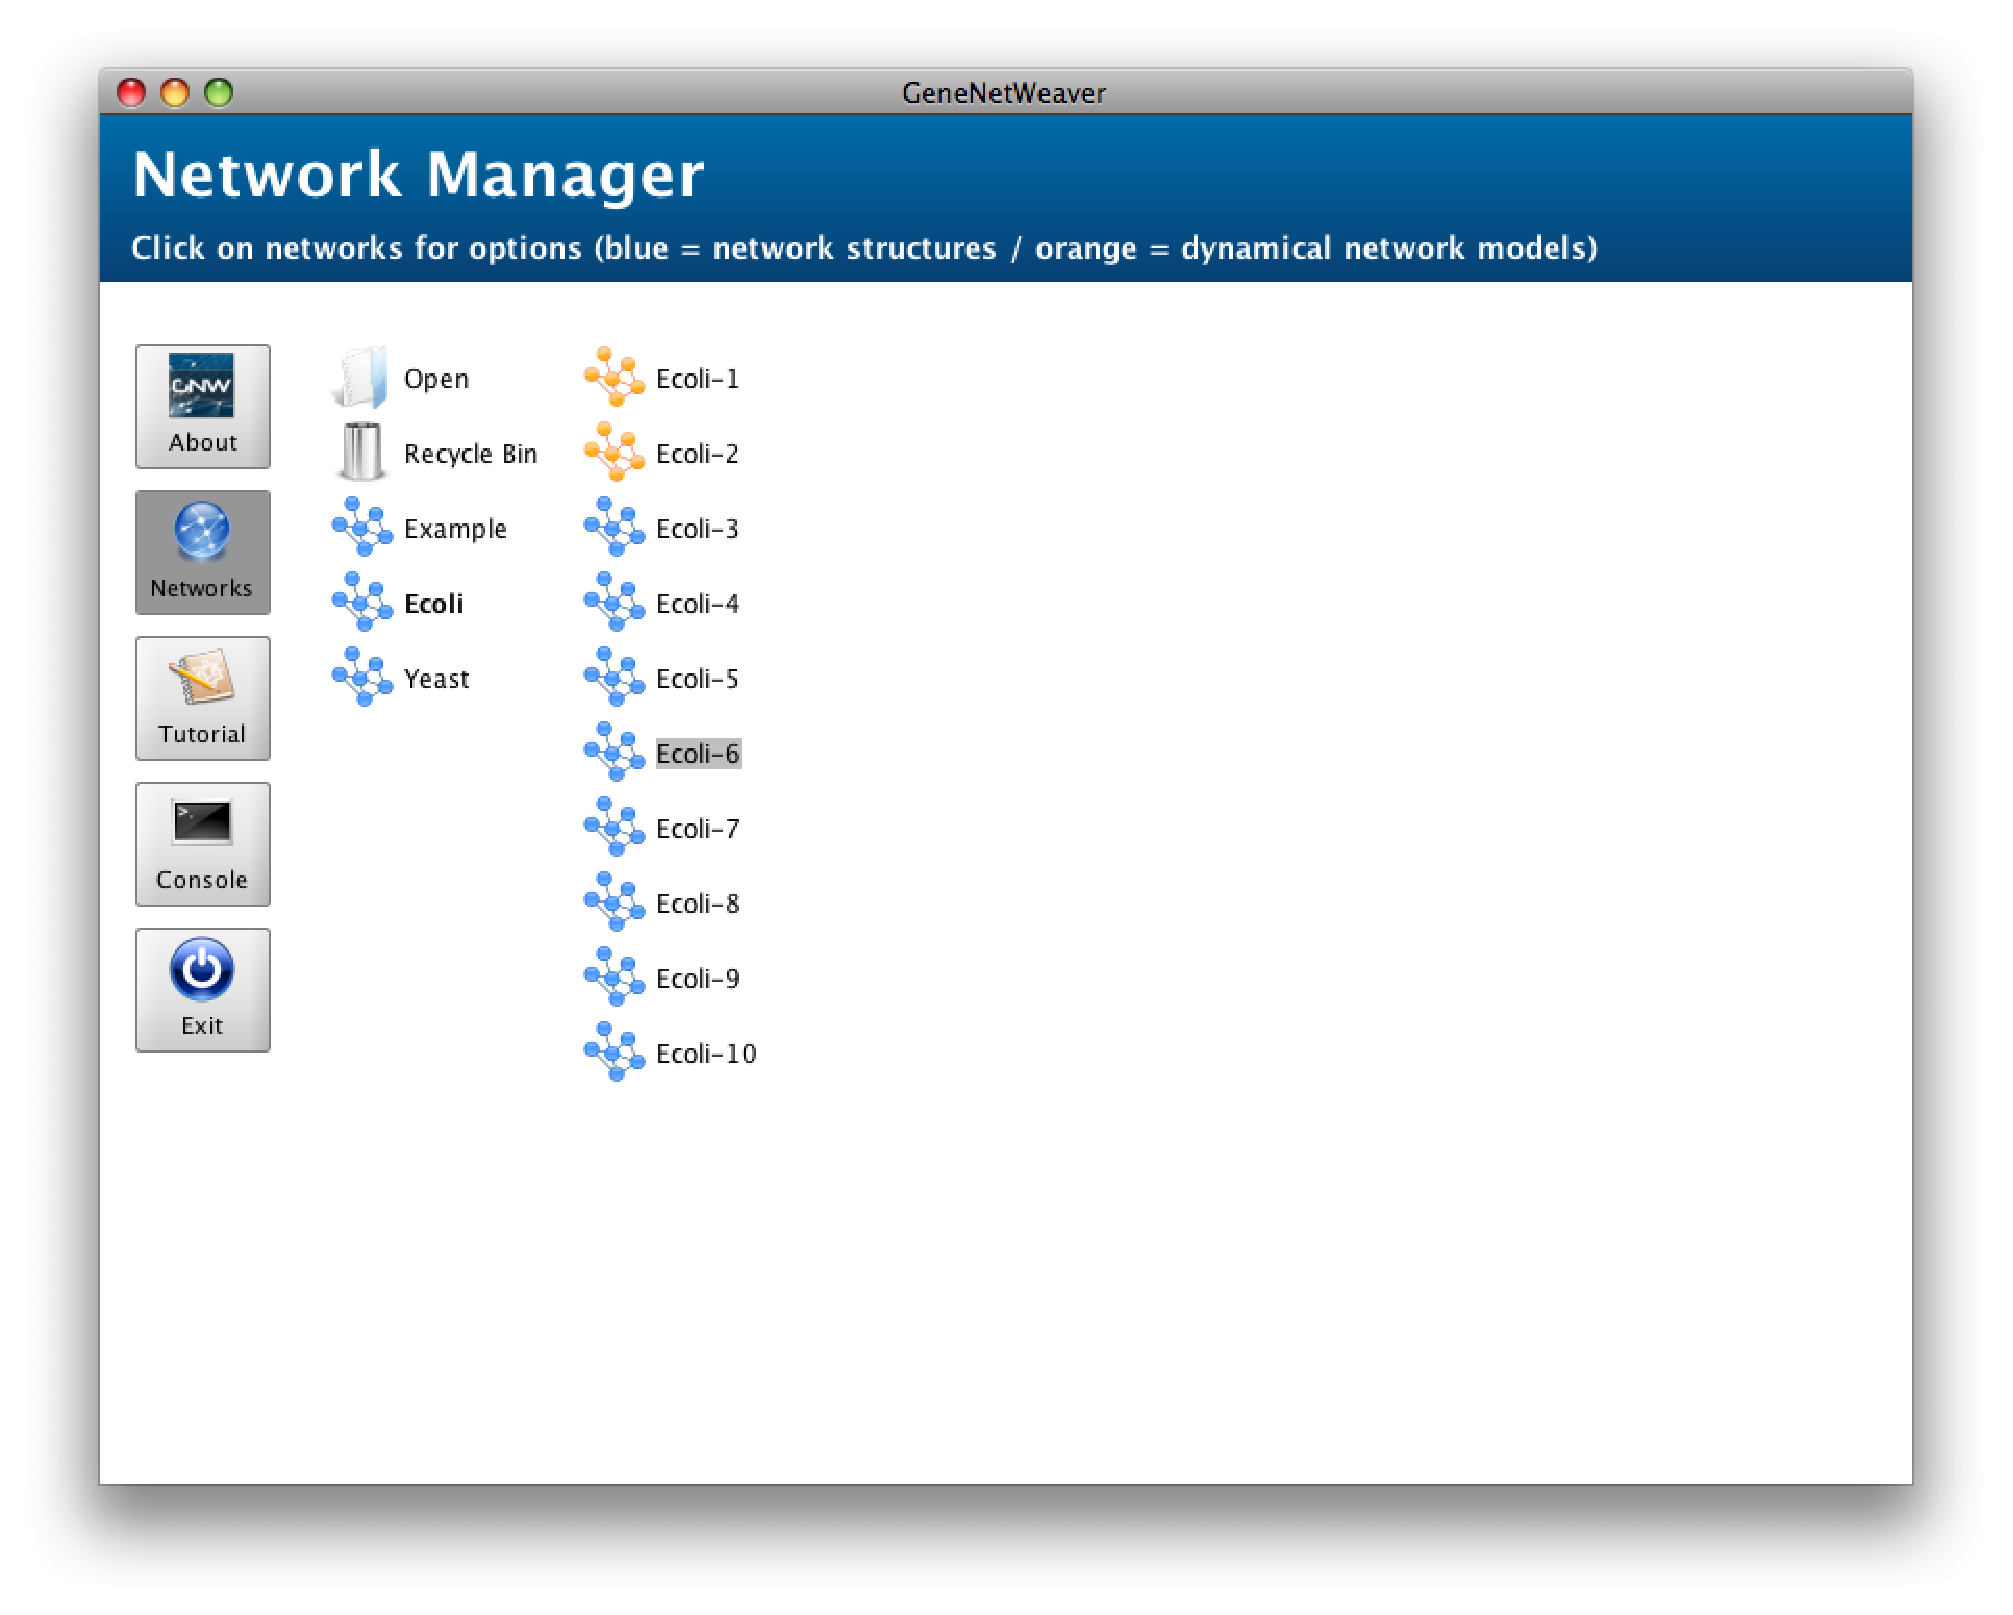
\includegraphics[width=9.8cm]{figures/network-manager}
\caption{The \emph{Network Manager}}
\label{network-manager}
\end{figure}


\subsection{Automatically loaded networks}
\label{loaded-networks}

Three network structures are automatically loaded when GNW is started:
\begin{mylist}
 \item \textbf{Example}\\
 Hierarchical scale-free network model: 64 nodes, 207 edges. This network has a scale-free topology with embedded modularity similar to many biological networks (Ravasz et al. 2002. \emph{Science}, 297:1551-55).\\
 \item \textbf{Ecoli (signed)}\\
 E.coli transcriptional regulatory network: 1502 nodes, 3587 edges. Corresponds to the TF-gene interactions of RegulonDB release 6.2. (Gama-Castro et al. 2008. \emph{Nucleic Acids Res}, 36:D120-4). Note that this is a signed network and dynamical models will be initialized accordingly as described in Sect. \ref{dynamics}.\\
 \item \textbf{Yeast}\\
 Yeast transcriptional regulatory network: 4441 nodes, 12873 edges. As described by Balaji et al. (\emph{J Mol Biol}, 360:213-27, 2006).
\end{mylist}


% ==================================================================================

\section{Opening and saving network structures and dynamical models}
\label{opensave}

\subsection{Opening networks}

To import a network, double-click the \emph{Open} icon of the \emph{Network Manager} and use the dialog to browse your folder and open a file. If you click on the field \emph{Files of Type} of the \emph{Open} dialog, a list of the different network file formats supported by GNW will appear (see Fig. \ref{opendialog}). You can open network structures saved in TSV, GML, and DOT format. For dynamical models SBML is used\footnote{In the current version, only SBML files that have been generated by GNW can be opened.}. See the next section for a description of these formats. If the network is successfully parsed, a new network icon will appear in the Network Manager.\\

\textbf{Tip}: press the key \emph{O} from the \emph{Network Manager} to display the \emph{Open} dialog.\\

\begin{figure}[tbh]
\label{opendialog}
\centering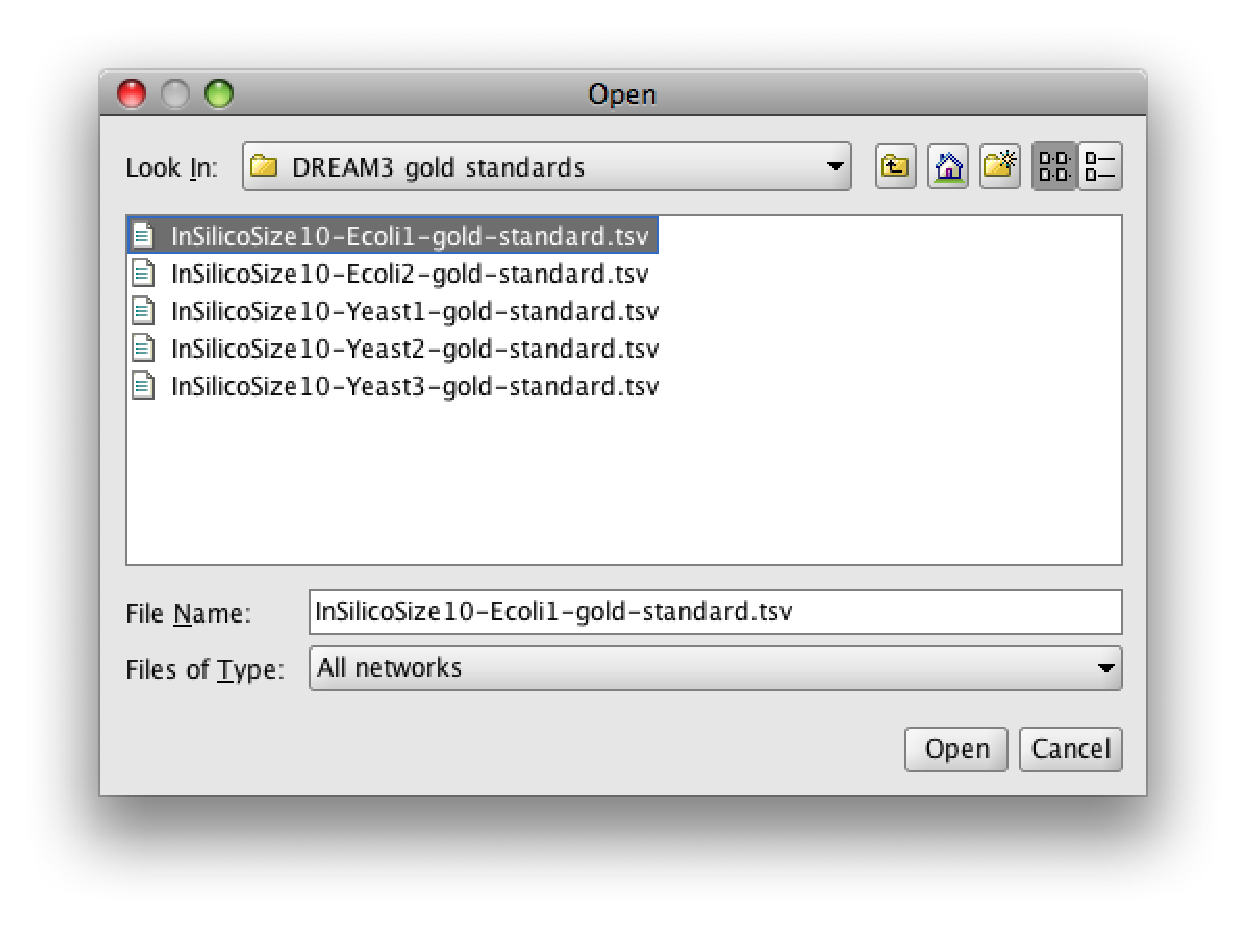
\includegraphics[width=9cm]{figures/open-dialog}
\caption{Double-clicking the \emph{Open} icon in the \emph{Network Manager} opens this dialog, which allows you to import network structures or dynamical networks.}
\end{figure}

\textbf{Important}: the filenames must end with the correct extension, otherwise they are not visible in the \emph{Open} dialog and GNW will refuse to load them. The recognized extensions are .tsv, .gml, .dot and .xml (since SBML is based on XML).

\subsection{Saving networks}

After having extracted subnetworks, you probably want to save them for later use. To export networks from GNW, double-click the icon of the network and select the option \emph{Export Network}. A dialog appears that allows you to specify a filename and to select a file format before saving the network. SBML format is only available for dynamical networks (as mentioned above, the SBML format that GNW uses is not yet compatible with other simulators).\\

\textbf{Note}: after simulating experiments, the networks will be automatically saved as described in Section \ref{experiments}. Thus, there is no need to save the networks manually before simulating experiments.\\

\textbf{Tip}: press the key \emph{S} from the \emph{Network Manager} to display the \emph{Save As} dialog.


% ==================================================================================

\section{Network file formats}

As mentioned in the previous section, there are two types of networks in GNW: \emph{network structures} and \emph{dynamical networks}. GNW supports TSV (tab-separated-values), GML (Graph Modelling Language) and DOT for network structures. DOT is the file format used by Graphviz, which is a useful software package for graph visualization\footnote{http://www.graphviz.org}. For dynamical networks, SBML (Systems Biology Markup Language) is used.\\

Network structures can be \emph{signed} or \emph{unsigned}. Unsigned networks are directed graphs without any information on the regulatory effect (enhancing or inhibitory) of interactions. In signed networks, the regulatory effect of interactions is specified. The type of interaction is in general either enhancing (+) or inhibitory (--).

\subsection{TSV format}
\label{tsv-formats}
This format is the easiest way to describe a network structure in GNW. Each line corresponds to a regulatory interaction from a source node (the regulator) to a target node. A line is composed of the following elements, separated by a tabulation:
\begin{mylist}
 \item Source node
 \item Target node
 \item Attribute (optional)
\end{mylist}
Both \emph{source} and \emph{target} nodes are represented by an identifier (string), and the optional \emph{attribute} is used to specify the type of the interaction. There are two different flavors of the TSV format for signed and unsigned network structures:
\begin{mylist}
\item \textbf{TSV network structure (*.tsv)}\\Should be used to save \emph{signed} network structures. The attribute is either `+' (enhancing), `$-$' (inhibitory), `+$-$' (dual), `?' (unknown), or `0' (zero). Note, if the value for the attribute is omitted, the interaction is assumed to be of type unknown.\\
 \item \textbf{DREAM gold standard network structure (*.tsv)}\\This is the file format used for the network structures in the DREAM challenge (the gold standards). The networks are \emph{unsigned}, thus there is no attribute. Optionally, the attribute may be set to `1' (present links) or `0' (absent links).
\end{mylist}

\textbf{Important}: It is usually not necessary to list the absent links (attribute `0') because links that are not listed are automatically assumed to be absent. We allow for the possibility to explicitly list the absent links for compatibility with the format used in the DREAM challenge. Also, it allows to add nodes to the network that have no connection. For example, the line ``\texttt{A  A  0}'' will add the node \texttt{A} with no connections to the network.

\subsubsection{Examples.} Consider a network with three nodes G0, G1, G2, with an interaction from G0 to G1 and from G0 to G2. This network can be described in TSV format by
\begin{verbatim}
G0   G1
G0   G2
\end{verbatim}
If we want to represent the same network, but with the first link enhancing and the second link inhibitory, we would use
\begin{verbatim}
G0   G1   +
G0   G2   -
\end{verbatim}
Note that when opening a network in TSV format, GNW automatically detects whether the network is signed or not.

\subsection{GML format}
GML, the \emph{Graph Modelling Language}\footnote{http://www.infosun.fim.uni-passau.de/Graphlet/GML}, is a common standard to describe network topologies. In GML, nodes and edges are defined separately. The following code describes the network used as example in the previous section using GML instead of TSV format.
\begin{verbatim}
graph [
   comment "GML syntax example"
   node [ id 0 label "G0" ]
   node [ id 1 label "G1" ]
   node [ id 2 label "G2" ]
   edge [ source 0 target 1 value "+" ]
   edge [ source 0 target 2 value "-" ]
]
\end{verbatim}
For signed networks, the interaction types are specified by the field \emph{value} using the same attributes as defined in the previous section. For unsigned networks, you can simply omit the \emph{value} field of the interactions (if no value is given, the interaction type is considered to be \emph{unknown}). Note that the \emph{comment} field is ignored by GNW. 


\subsection{DOT format}
\label{dotformat}
DOT is yet another standard graph description language. Similar to GML, networks are described by separately defining nodes and edges with several attributes for each of them. DOT files are used with the Graphviz\footnote{http://www.graphviz.org} softwares (Dot, Neato, etc.) to obtain a representation of the graph as image (PNG, PDF, EPS, etc.). Only a small part of the features of the DOT language are used by GNW. The example below shows the code for the network described in the previous sections, this time in DOT format
\begin{verbatim}
digraph [
   "G0";
   "G1";
   "G2";
   "G0" -> "G1" [value="+"];
   "G0" -> "G2" [value="-"];
]
\end{verbatim}
The \emph{value} field is used by GNW as explained in the previous section for the GML format.

\subsection{SBML format}
The Systems Biology Markup Language (SBML) is a standard format to represent dynamical models of biological systems. GNW uses SBML to open/save dynamical networks. For a detailed description of SBML, please refer to the web site of the SBML project\footnote{http://www.sbml.org}.\\

\textbf{Important}: currently GNW does not produce files that are compatible with other simulators, and you cannot open SBML files from other simulators with GNW. We intend to address this issue in the next version of GNW, at that time we will also provide a more detailed description.


% ==================================================================================

\section{Visualizing networks}

GNW has an easy-to-use interface to visualize the networks that you have imported or generated with the subnetwork extraction method. The visualization is based on the excellent Java library JUNG (Java Universal Network/Graph Framework), an open-source project available on SourceForge.net\footnote{http://jung.sourceforge.net}. To visualize a network from the \emph{Network Manager}, double-click it and choose \emph{Visualization}.\\

\textbf{Tip}: press the key \emph{V} or use the third/middle button of your mouse to open the graph visualization window directly from the \emph{Network Manager}.\\

\textbf{Warning}: visualization is mainly thought for medium or small networks (less than 1000 nodes). You can try to visualize larger networks, but it may take a long time and the graph layout probably won't be be well arranged.\\

\textbf{Tip}: alternatively, you can export your network in DOT format and use Graphviz or other professional tools for graph visualization (see Section \ref{dotformat}).\\

\begin{figure}[tbh]
\centering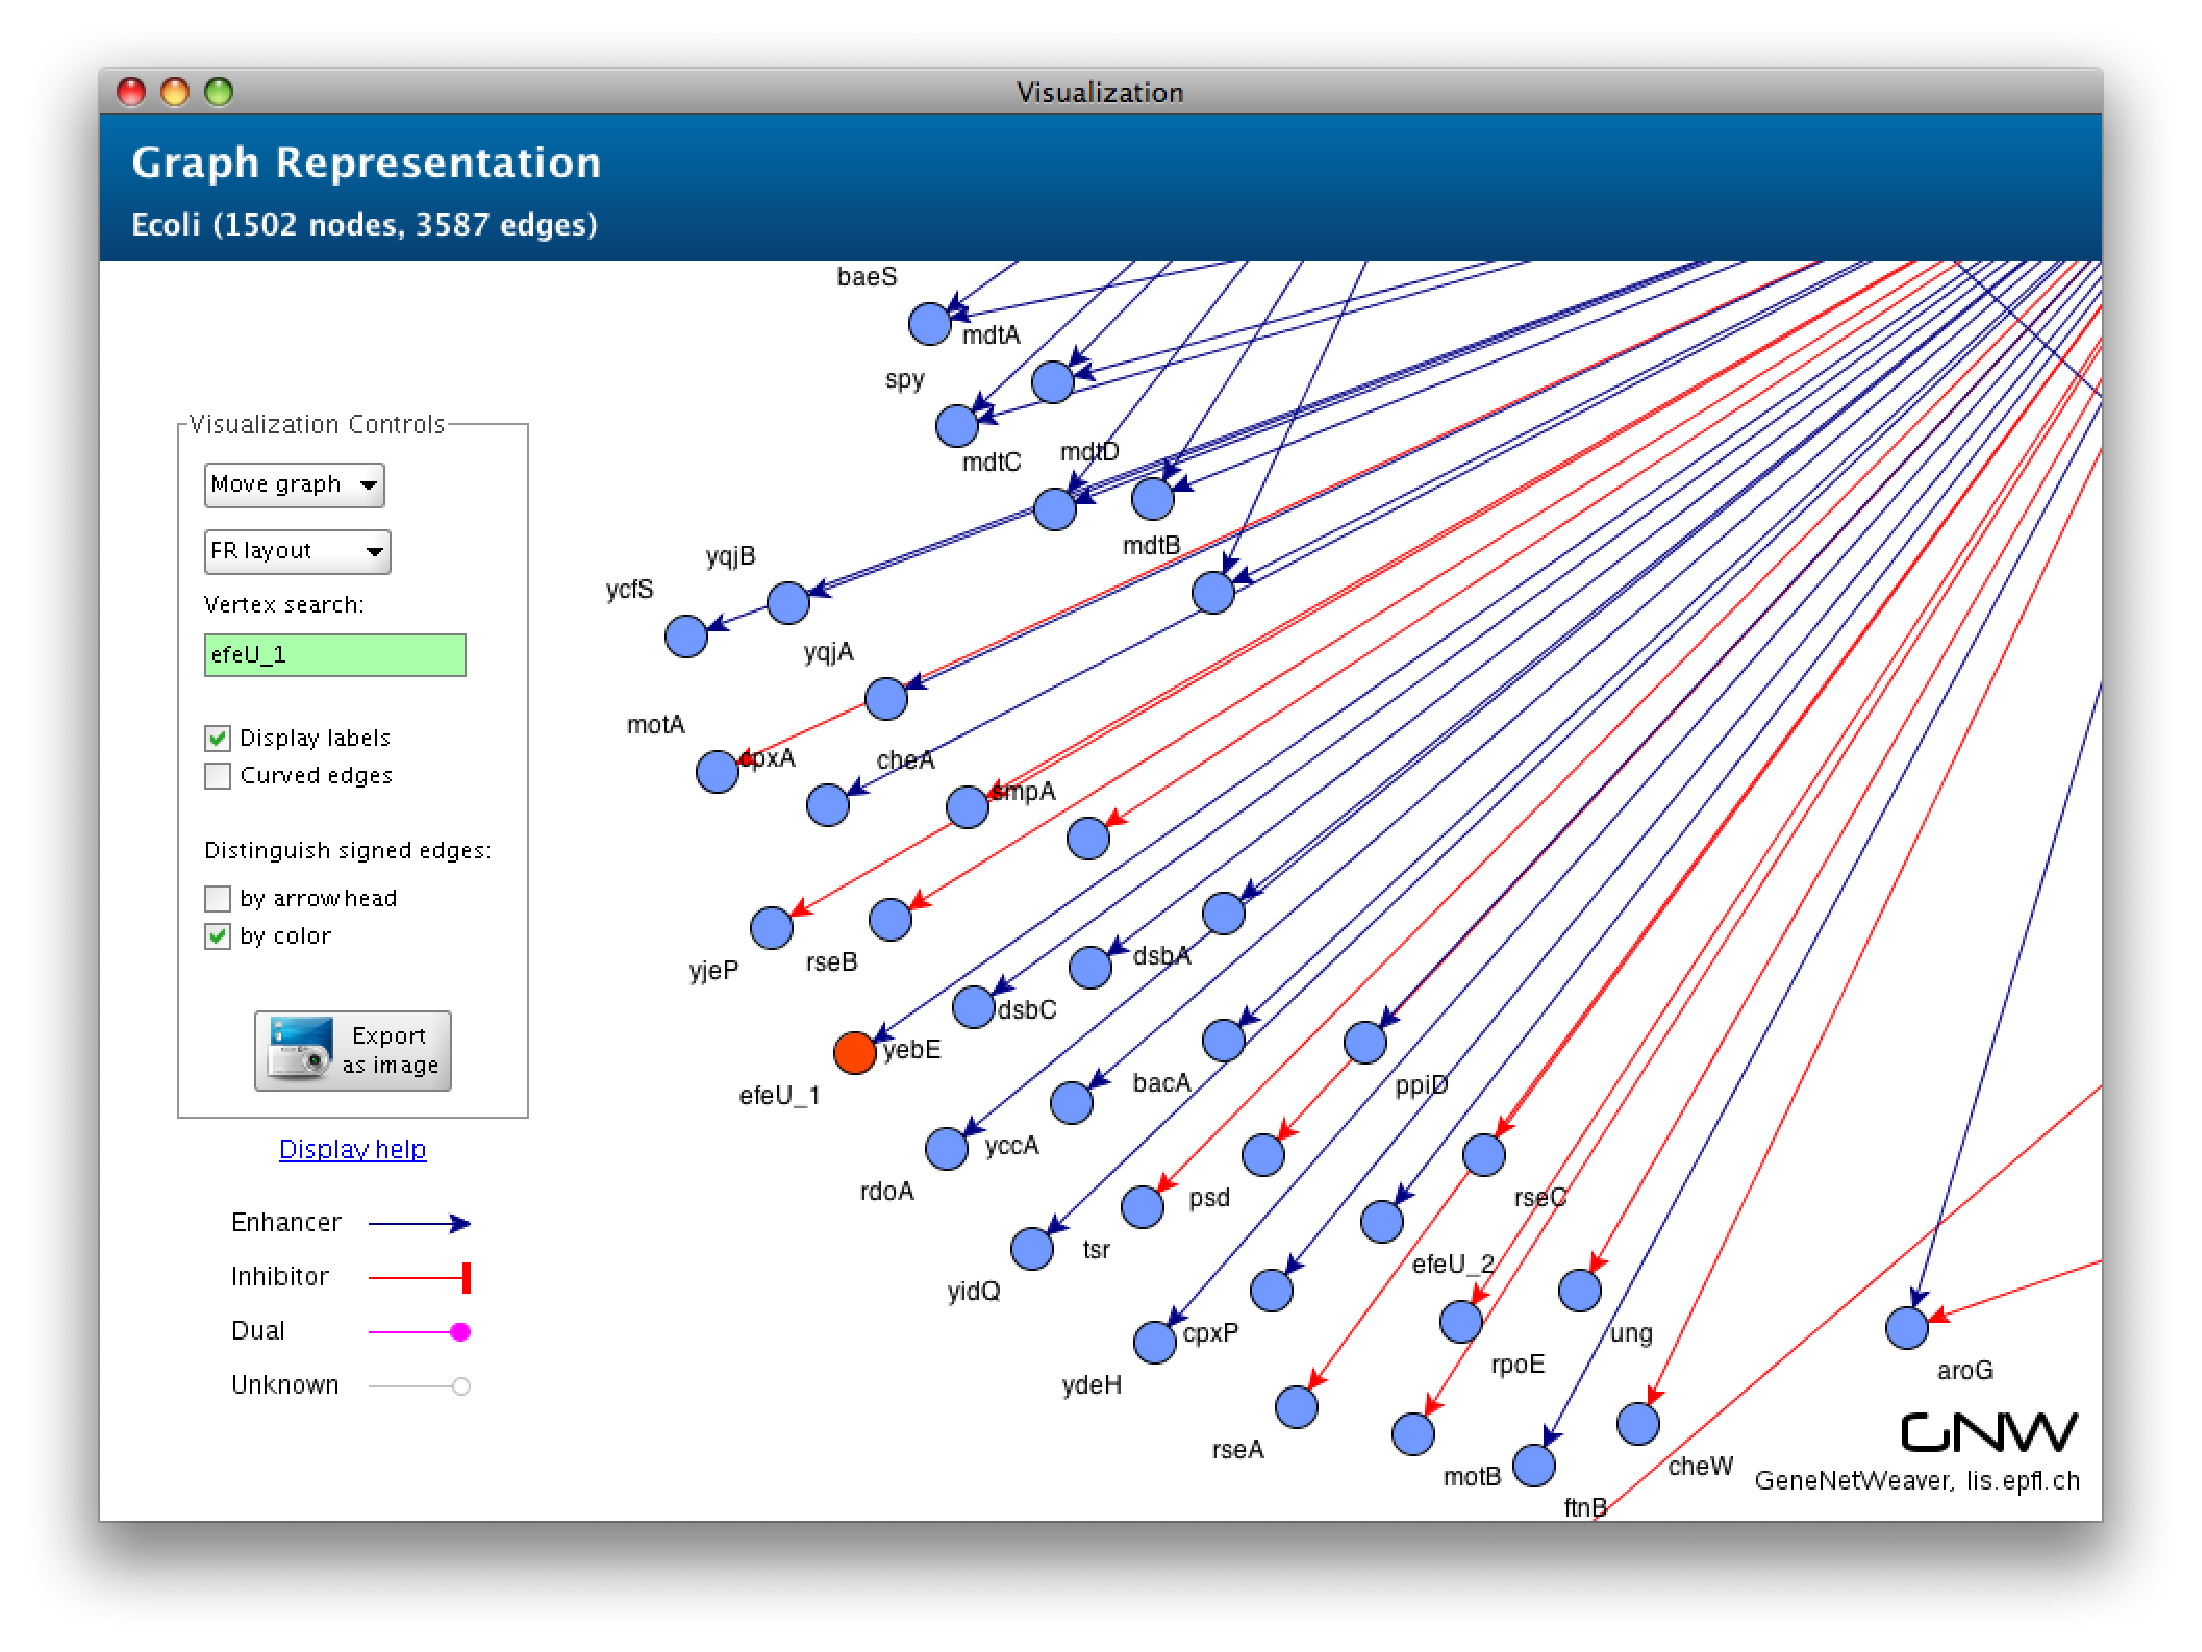
\includegraphics[width=10.6cm]{figures/visualization}
\caption{The GNW network visualization interface.}
\label{visualization}
\end{figure}

Click and drag to move the graph around, and use the scroll wheel to zoom in our out. Use the link \emph{Display help} in the visualization window for information on additional actions (e.g., rotation) that you can perform on the graph.\\

The \emph{Visualization Controls} panel in the left part of the visualization window allows to change and manipulate the graph representation in a number of ways:
\begin{mylist}
 \item \textbf{Move graph/nodes}\\In \emph{move graph} mode, you can move the whole graph using the left mouse button. In the \emph{move nodes} mode you can move one or several nodes, which is useful if the automatic graph layout is not optimal.\\

 \item \textbf{Graph layouts}\\Three different layouts allow to change the way the nodes are distributed:
	\begin{itemize}
	 \item Kamada-Kawai algorithm (force-based)
	 \item Fruchterman-Reingold algorithm (force-based)
	 \item Positions vertices equally spaced on a regular circle.\\
	\end{itemize}
 
 \item \textbf{Vertex search}\\Searching a specific node in a network with thousands of nodes is like looking for a needle in a haystack! \emph{Vertex search} helps you to find a node or group of nodes according to their labels. If an entered string corresponds exactly to the label of a node, the node is highlighted red and the search field becomes green. If the entered string partly matches several node labels, these nodes will appear in orange. If the string matches no label, the search field will become red.\\
 
 \item \textbf{Display labels}\\If checked, the labels of the nodes are displayed.\\
 
 \item \textbf{Curved edges}\\If checked, the interactions are represented by curved edges instead of straight lines.\\
 
 \item \textbf{Distinguish signed edges:}
	\begin{itemize}
	 \item \textbf{by arrow head}\\If checked, signed interactions have different arrow heads depending on their type, as shown in the legend in the bottom left corner of the visualization window (see Figure \ref{visualization}). If the network is unsigned, all the interactions are of type \emph{unknown}.\\
	 \item \textbf{by color}\\If checked, signed interactions are colored as shown in the legend mentioned above. If the network is unsigned, all the interactions are of type \emph{unknown}.\\
	\end{itemize}
 \item \textbf{Export as image}\\Take a snapshot of the graph. The network can be exported in JPEG, PNG, and EPS image formats.
\end{mylist}



% ==================================================================================

\section{Extracting subnetworks from a source network}

\textbf{Important}: we assume that you have read our paper \citep{Marbach2009}, which describes and motivates the subnetwork extraction method for generating reverse engineering benchmarks.\\

Click the \emph{Networks} button in the main window of GNW to enter the \emph{Network manager}. Double-click the source network from which you want to extract subnetworks. Click \emph{Subnetwork extraction} to open the subnet extraction dialog, which allows you to set the different parameters for the extraction. We will now explain each of the fields of this dialog:

\begin{mylist}

\item \textbf{Subnets name}\\The prefix of the name of the subnets. If you enter the name \emph{subnet}, the extracted subnetworks will be named \emph{subnet-1}, \emph{subnet-2}, etc.\\

\item \textbf{Number of subnets}\\The number of subnetworks that you want to extract.\\

\item \textbf{Seed}
\begin{itemize}
\item \textbf{Random vertex}\\
For each subnet, the extraction method starts from a different randomly picked seed node of the source network.\\
\item \textbf{Selection from list}\\
Select the seed node manually from the list of all nodes of the source network.\footnote{Note, if you extract several subnetworks from the same seed, they are usually very similar, but not necessarily identical. They are not identical because if in the subnetwork extraction process several neighboring nodes lead to the same modularity, one of them is chosen randomly.}\\
\end{itemize}

\item \textbf{Neighbor selection}

\begin{itemize}
\item \textbf{Greedy}\\
In the subnetwork extraction process, always choose the neighboring node for addition that maximizes the modularity (if several neighbors lead to the same modularity, one of them is chosen randomly).\\
\item \textbf{Random among top (\%)}\\
Specify a percentage $p$. Instead of always adding the neighboring node that maximizes the modularity, one of the top $p$\% neighbors with the highest modularity is chosen randomly. The effect of this parameter is discussed in the methods section of \citet{Marbach2009}: varying $p$ between 0\% and 100\% allows for tuning of the sampling strategy from pure modular subnetwork extraction to random subnetwork extraction. We usually use either the greedy strategy or $p=10\%$ to add some stochasticity.
\end{itemize}

\end{mylist}

Click \emph{Extract} to run the subnetwork extraction. This may take a minute for large networks. You can see the order in which neighboring nodes are added to the subnetwork in the console, along with the modularity at each step.\\

\textbf{Tip}: press the key \emph{E} from the \emph{Network Manager} to display the \emph{Subnetwork Extraction} dialog.


% ==================================================================================

\section{Random initialization of dynamics}
\label{dynamics}

Click the \emph{Networks} button in the main window of GNW to enter the \emph{Network manager}. Double-click the network structure (network structures have blue icons) that you want to convert into a dynamical network model. Usually this is a subnetwork that you have previously extracted as described in the previous section.\\

Click \emph{Random initialization of dynamics}. In the dialog, leave the checkbox checked if you want to remove autoregulatory interactions (self-loops). Otherwise, uncheck it. If your network has no autoregulatory interactions, this option has no effect.\\

For the DREAM challenges, we have removed autoregulatory interactions for the following reason. A first class of reverse engineering methods cannot identify autoregulatory interactions and will consequently set them all to zero per default. A second class of methods tries to infer autoregulatory interactions, but in our experience this is quite difficult. Since overall, there are few autoregulatory interactions in the transcriptional networks that we considered, paradoxically the first class of methods would actually perform well: since they set all autoregulatory interactions to zero, and a large majority are indeed zero, the performance is actually very good. In contrast, the methods that try to infer the few autoregulatory interactions risk to have many false positives. In order not to favor the first or the second class of methods, we did not ask participants to predict autoregulatory interactions and removed them from the DREAM challenge networks.\\

\textbf{Important}: for signed network structures, the dynamics are initialized such that the signs in the dynamical network are the same as in the original network structure. In other words, excitatory / inhibitory interactions will be initialized such that they actually have an excitatory / inhibitory effect in the dynamical model. For unsigned network structures, the signs in the dynamical model are initialized arbitrarily.\\

We are currently working on two papers describing the dynamical model and its initialization in detail. Note that the initialization is done such that the created regulatory dynamics are somewhat biologically plausible. We have also verified the dynamical model on \invivo data. We will update this section as soon as possible. In the meantime, you may contact us for a draft of the model description.\\


% ==================================================================================

\section{Simulation of experiments}
\label{experiments}

Click the \emph{Networks} button in the main window of GNW to enter the \emph{Network manager}. Double-click the dynamical model (dynamical networks have an orange icon) that you want to simulate to produce datasets. Click \emph{Simulate experiments}. In the dialog that pops up, you can specify the type of experiments and the amount of noise that you want to add to the data:

\begin{mylist}

\item \textbf{Experiments}

\begin{itemize}

\item \textbf{Steady-state for wild-type and null-mutants}. GNW will compute the steady-state for the wild-type (the unperturbed network) and for the gene knockouts. For a network of size $N$, there are $N$ knockout experiments. In the $k$'th knockout experiment, the transcription rate of gene $k$ is set to zero (the gene is deleted) and the resulting steady-state is computed\footnote{The steady-state concentration of the gene that is knocked out is zero. However, after adding noise the concentration will be non zero (you may interpret that as measurement error).}.\\

\item \textbf{Steady-state for wild-type and heterozygous knock-down strains}. GNW will compute the steady-state for the wild-type\footnote{If both the null-mutants and the heterozygous knock-down strains are selected, the wild-type is only computed once.} and for heterozygous knock-down strains. In the $k$'th knock-down experiment, the maximum transcription rate of gene $k$ is divided by two as compared to the wild-type\footnote{In a diploid cell, this can experimentally be achieved by deleting one of the two copies of a gene. In a haploid cell, the terminology ``heterozygous knock-down'' above is incorrect, but a similar effect could be achieved with other experimental means (e.g., siRNA).}.\\

\item \textbf{Trajectories from wild-type to perturbed steady-state}. You can save the trajectories from the wild-type to the new steady-state in the perturbation experiments described above. At time t=0 the wild-type steady-state is given. At that time, the perturbation is applied (the expression rate of a gene is set to zero [null-mutant] or reduced by half [heterozygous knock-down]). The trajectory shows how the network goes to the new steady-state. You can set the number of time points and the duration of the trajectories in the Settings described below. Note that these settings do not affect the computation of the steady-states, they only determine which time points will be saved in the exported dataset (the integration for the steady-state computation continues beyond the duration of the trajectory if necessary). To find out what is a reasonable duration for the trajectories, run the simulation and observe the output on the console, which indicates for each knock-out / knock-down when the true steady-state is reached.\\

\item \textbf{Time series experiments}. Select the number of time series that you want to produce. The duration and number of time points of each time series can be set in the Settings below. The time series data shows how the networks recover from external perturbations. Trajectories are simulated by integrating the networks from a different randomly perturbed initial condition for every time series (only the initial conditions change, the network structure and parameters remain constant). The initial conditions are obtained by adding a random number from a normal distribution to the wild-type steady-state. The number of time points does not affect the precision of the numerical integration, this is just the number of time points that will be saved in the dataset.\\

\end{itemize}

\item \textbf{Settings}

\begin{itemize}

\item \textbf{Number of time points / duration of each time series}. Set the number of time points and the duration of the trajectories. The time step is set according to these values. As mentioned above, these settings do not affect the precision of the integration.\\

\item \textbf{Noise}. Check this box to add noise to the simulated data. You can specify the standard deviation of the Gaussian noise. The simulation remains deterministic, the noise is added afterwards to the simulated data.\footnote{Concentrations that become negative due to noise are clipped at zero. We choose this because it's the most simple way to add noise. We spent quite some time thinking about more realistic ways to add noise, e.g. using a mix of normal and log-normal noise, but realized that anything more advanced than Gaussian would have to be justified by modeling a specific experimental technology (e.g. microarrays, q-PCR, etc.). However, we chose not to model any specific technology to stay as general as possible.}\\

\item \textbf{Output directory}\\ GNW will automatically save all relevant files of the benchmark (the simulated datasets, the network structure, the dynamical model of the network, etc.) in the output directory specified here. See the next section for a description of the exported files.\\

\end{itemize}

\end{mylist}

After clicking \emph{OK}, GNW will simulate the experiments and save the files described in the next section in the specified output directory.\\

\textbf{Tip}: press the key \emph{B} from the \emph{Network Manager} to display the \emph{Experiments Simulation} dialog (only with dynamical models).

\subsection{Description of exported files}

GNW uses different file types to save network structures, dynamical network models, and various types of data from simulated experiments. All files except the dynamical network model are saved in tab separated value format (TSV). These are text files that you can open and edit with any text editor or Excel, for example. Note that you can easily convert .tsv format into the sometimes preferred comma separated value format (CSV) by using the \emph{search and replace} function of your text editor to replace all tabs with commas.\\

In the next sections we describe the format of all files that are saved by GNW automatically after the simulation of experiments.

\subsubsection{Unsigned network structure / DREAM gold standard.}
GNW saves the unsigned network structure in a file called \emph{ $<$name$>$-gold-standard.tsv}, where \emph{ $<$name$>$} is the name of the network in the \emph{Network Manager}. The file is in TSV format and can subsequently be opened with GNW as described in Section \ref{opensave}. For each regulatory link from a gene \texttt{A} to a gene \texttt{B} there is a line ``\texttt{A   B   1}'' in the file.\\

Note: To save space, we do not list all the zero connections as done in the DREAM3 gold standards. Consequently, the evaluation script to compute the scores of a prediction available from the DREAM website gives an error. You should use the adapted version of this script instead, which is available on our website (gnw.sf.net).

\subsubsection{Signed network structure.}
The signed network structure is saved in the file \emph{ $<$name$>$-gold-standard-signed.tsv}. The file can be opened with GNW as described in Section \ref{opensave}. For each regulatory link from a gene \texttt{A} to a gene \texttt{B} there is a line ``\texttt{A B} \emph{$<$sign$>$}'', where \emph{$<$sign$>$} is `+' if the interaction is enhancing and `--' if the interaction is inhibitory. We don't provide a script to evaluate signed predictions, but one could use the same approach as in DREAM2.

\subsubsection{Dynamical network model.}
The dynamical network is saved to the file \emph{ $<$name$>$.xml} in SBML format. These files can be opened and simulated with GNW. However, currently these files cannot be opened with other simulators than GNW. A more compatible SBML export will be supported in the next version of GNW.

\subsubsection{Steady-state datasets.}

The null-mutant and the heterozygous knock-down data are saved to the files \emph{ $<$name$>$-null-mutants.tsv} and \emph{ $<$name$>$-heterozygous.tsv}, respectively. The first line of these files is the wild-type steady-state, followed by a new line for every knock-out / knock-down experiment. The columns correspond to the genes, as indicated by the lables in the header line. These files can be loaded and visualized in Matlab with the scripts described in Section \ref{m-files}. If noisy datasets are produced, GNW saves in addition the data before addition of noise in two separate files with the prefix \emph{nonoise}. Furthermore, the protein concentrations with and without noise are also saved in corresponding files with the prefix \emph{proteins}.

\subsubsection{Time series datasets.}
There are two types of time series experiments: (1) the trajectories from the wild-type to the null-mutant / heterozygous knock-down steady-states are saved to the files \emph{$<$name$>$-null-mutants-trajectories.tsv} and \emph{$<$name$>$-heterozygous-trajectories.tsv} (only if the corresponding checkbox has been selected in the simulation of the expriments); (2) The data of the other time series experiments is saved to the file \emph{ $<$name$>$-trajectories.tsv}. The format is the same for all time series datasets. Each line corresponds to a time point, the time is given in the first column. The following columns correspond to the genes as indicated in the header line. If several time series were produced, they are saved in the same file one after the other, separated by an empty line. In the trajectories from wild-type to the null-mutant / heterozygous knock-down, the $k$'th time series corresponds to the knockout / knock-down of gene $k$. Again, if noisy datasets are produced, GNW saves in addition the data before addition of noise in a file with the prefix \emph{nonoise}, and the protein concentrations with and without noise are saved in the files with the prefix \emph{proteins}.\\

The initial conditions for both mRNA and proteins for all time series are saved in the file \emph{ $<$name$>$-initial-conditions.tsv}. The first line corresponds to the first time series, and so on. The initial conditions are identical to the first time point of the trajectories without noise.


% ==================================================================================

\section{Visualization of data in Matlab}
\label{m-files}

We provide two m-files that can be used to load and visualize the steady-state and time series datasets in Matlab (available for download on gnw.sf.net):

\begin{mylist}
\item \textbf{dream3ss.m} is the script for the steady-state data. It loads and plots the null-mutant and heterozygous knockdown steady-state data produced by GNW using the Matlab function \emph{clustergram} (see Fig. \ref{dream3ss}). Check the Matlab documentation for \emph{clustergram} or type \emph{help dream3ss} for more information.\\

\item \textbf{dream3ts.m} is the script for the time series data. It loads and plots the time series data produced by GNW. Each time series is plotted in a separate figure. The profiles of the genes are clustered into groups as shown in Fig. \ref{dream3ts}. In Matlab, type \emph{help dream3ts} for more information.
\end{mylist}

\begin{figure}[tbh]
\label{dream3ss}
\centering\includegraphics[width=11cm]{figures/InSilicoSize10-Ecoli1-nonoise-ss}
\caption{Plotting the noisefree steady-state data from the network \emph{Ecoli1} of the DREAM3 challenge of size 10 with \emph{dream3ss}. On the top, the steady-state concentrations are shown. Values are normalized, thus concentrations range from 0 to 1 (see color bar on the right). Each row corresponds to a gene, and each column corresponds to an experiment. The first column is the wild-type steady-state. Then comes, for every gene, first the null-mutant and then the heterozygous knock-down experiment. The rows are clustered so that genes that have a similar expression pattern across the experiments are grouped together. For example, you can see that G2, G10, G8, and G9 (the top four rows) are constitutively active and have no inputs.
In the second plot, the difference to the wild-type is shown. Most squares are black, i.e., there is no difference to the wild-type. But you can see for example that if G10 is knocked out G7 is upregulated (red square in the bottom right corner), suggesting an inhibitory interaction from G10 to G7. You can also confirm this in the plot on the top (note that the order of the rows is different in the two plots).}
\end{figure}

\begin{figure}[tbh]
\label{dream3ts}
\centering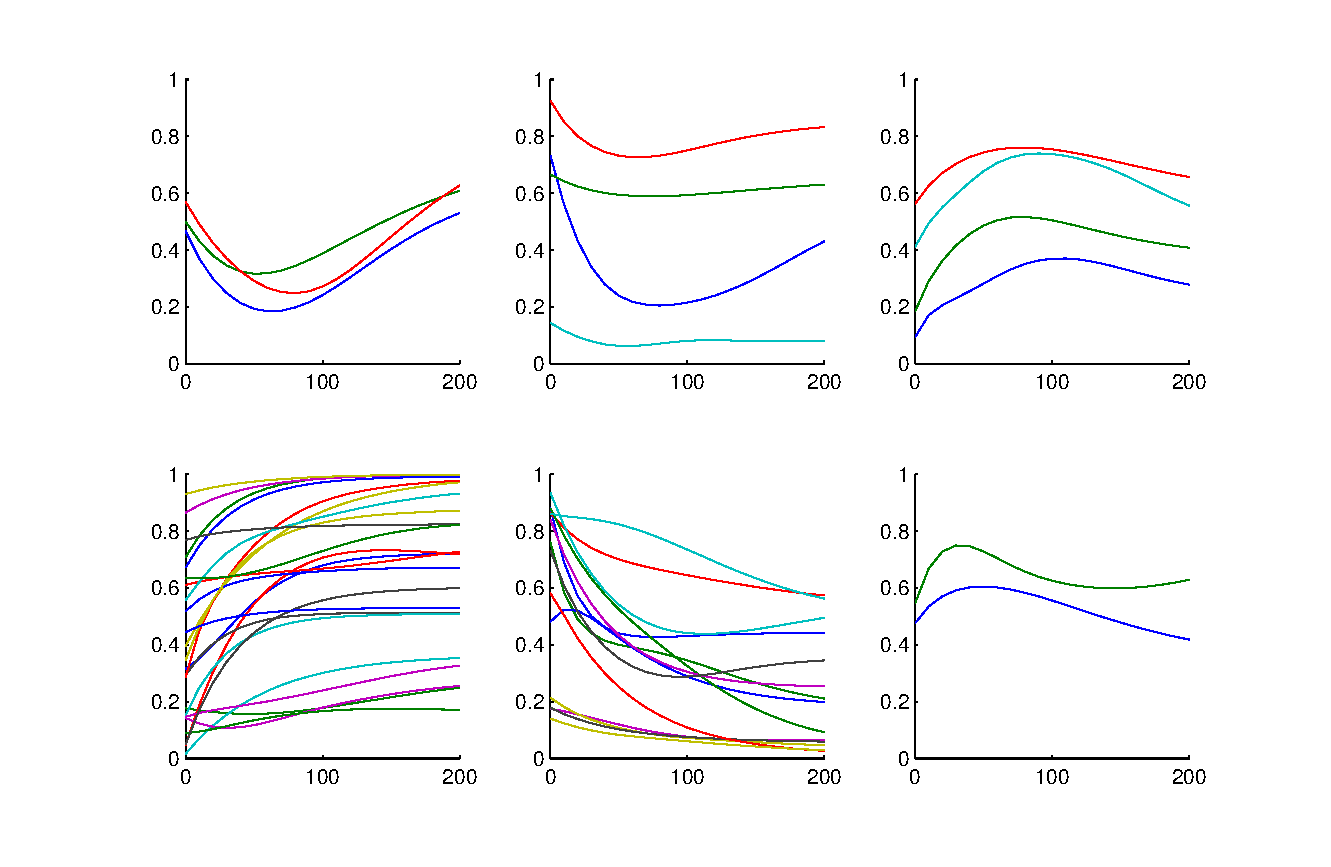
\includegraphics[width=\textwidth]{figures/InSilicoSize50-Yeast3-nonoise-ts}
\caption{Plotting one of the time series without noise from the network \emph{Yeast3} of the DREAM3 challenge of size 50 with \emph{dream3ts}. The colored lines are the trajectories of the 50 genes, grouped into 6 clusters. The y-axis is the normalized mRNA concentration and the x-axis is time.}
\end{figure}

% ==================================================================================

\section{Generating identical benchmarks as in DREAM3}
\label{gen-DREAM3-bench}

In this section we explain how you can generate \emph{exactly} the same type of benchmarks as used in DREAM3. First, you need to import the e.coli and yeast source networks that we used to generate the network structures in DREAM3 (these are not the same as the e.coli and yeast networks that are automatically loaded by GNW).\\

\textbf{Important}: We do not recommend to use these two source networks anymore and describe them here only for historical reasons. Instead, use the networks that are automatically loaded by GNW at start up (see Sect. \ref{loaded-networks}).\\

If you still want to use these networks, they are available in the file \emph{DREAM3 In Silico Challenges.zip} on our website (gnw.sf.net):
\begin{mylist}
\item \textbf{ecoli-ShenOrr2002.tsv}\\
The e.coli transcriptional regulatory network from Shen-Orr et al. (\emph{Nat Genet}, 31:64-68, 2002). The file corresponds to the updated version (1.1) without autoregulatory loops, taken from Uri Alon's website\footnote{http://www.weizmann.ac.il/mcb/UriAlon/Network\_motifs\_in\_coli/ColiNet-1.1}. (Note, in Shen-Orr's file the first column is the target and the second column is the regulator. We use the opposite convention. Thus, we reformatted the file. This is why the two files look different---but they correspond to the exact same network structure.) Compared to RegulonDB / EcoCyc network that is automatically loaded by GNW, the Shen-Orr network is not up to date anymore.\\

\item \textbf{yeast-Reguly2006.tsv}\\
A yeast genetic interaction network described in Reguly et al. (\emph{J Biol}, 5:11, 2006). In contrast to the yeast network that is automatically loaded by GNW, this is not a transcriptional network.
\end{mylist}

For subnetwork extraction, random seeds and neighbor selection from the top 10\% were used. Autoregulatory interactions were removed and noise with standard deviation 0.05 was added.


\section{Evaluating your predictions}

\emph{Precision-Recall} (PR) and \emph{Receiver Operator Characteristic} (ROC) curves are widely used to assess the performance of binary decision algorithms in the field of machine learning methods. Since inferring the structure of a network is a matter of deciding for each possible interaction if it is present or not, PR and ROC curves can be used to assess the performance of network reverse engineering algorithms. In the DREAM challenges, algorithms are assessed based on the area under the PR and ROC curves (AUPR and AUROC). PR and ROC are closely related, see \citet{Davis2006} for a good discussion. \\

On our website (gnw.sf.net) we provide a modified version of the Matlab evaluation script of the DREAM challenges (written by G.A. Stolovitzky, B. Jagla, and R. Prill). The file is called \emph{evaluation.m} and can be used to plot the PR / ROC curves and compute AUPR / AUROC scores. The script takes as input a gold standard file, a prediction file, and the size of the network. Type \emph{help evaluation} in Matlab for further information.\\

The gold standard file must be formated as follows:
\begin{verbatim}
G0   G1   1
G0   G2   1
...
G1   G0   0
...
\end{verbatim}
Each line defines an interaction oriented from the first gene to the second gene. The third element is 1 if the interaction is present in the gold standard and 0 otherwise. Instead of listing the absent (0) interactions, they can also simply be omitted (see also Sect. \ref{tsv-formats}). In this case, the size of the network (i.e., the number of genes) must be passed as an argument to \emph{evaluation.m}.\\

The format for the predictions is the same as used for the DREAM challenges:
\begin{verbatim}
G0   G1   0.98
G0   G2   0.8
...
G1   G0   0
...
\end{verbatim}
As in the gold standard file, each line defines an interaction oriented from the first to the second gene. For each interaction, a \emph{confidence level} between 0 and 1 is given that indicates the degree of belief that the interaction is included in the gold standard. The predictions must be listed in \emph{descending} order relative to their confidence level (the first prediction in the list is the one that you are most sure of). The confidence levels are only used to verify that the list of predictions is correctly ordered, they do not affect the PR and ROC curves and the evaluation in any other way. See the DREAM website\footnote{http://wiki.c2b2.columbia.edu/dream/index.php/The\_DREAM3\_In-Silico-Network\_Challenges.\_Description} for additional information. \citet{Marbach2008} discuss different strategies for deriving confidence levels from standard network predictions. \\

The script doesn't take into account autoregulatory interactions and simply ignores them if they are present in the gold standard and/or in the list of predictions (the DREAM3 In Silico Challenges had no autoregulatory interactions).

\begin{figure}[tbh]
\label{PR-ROC}
\centering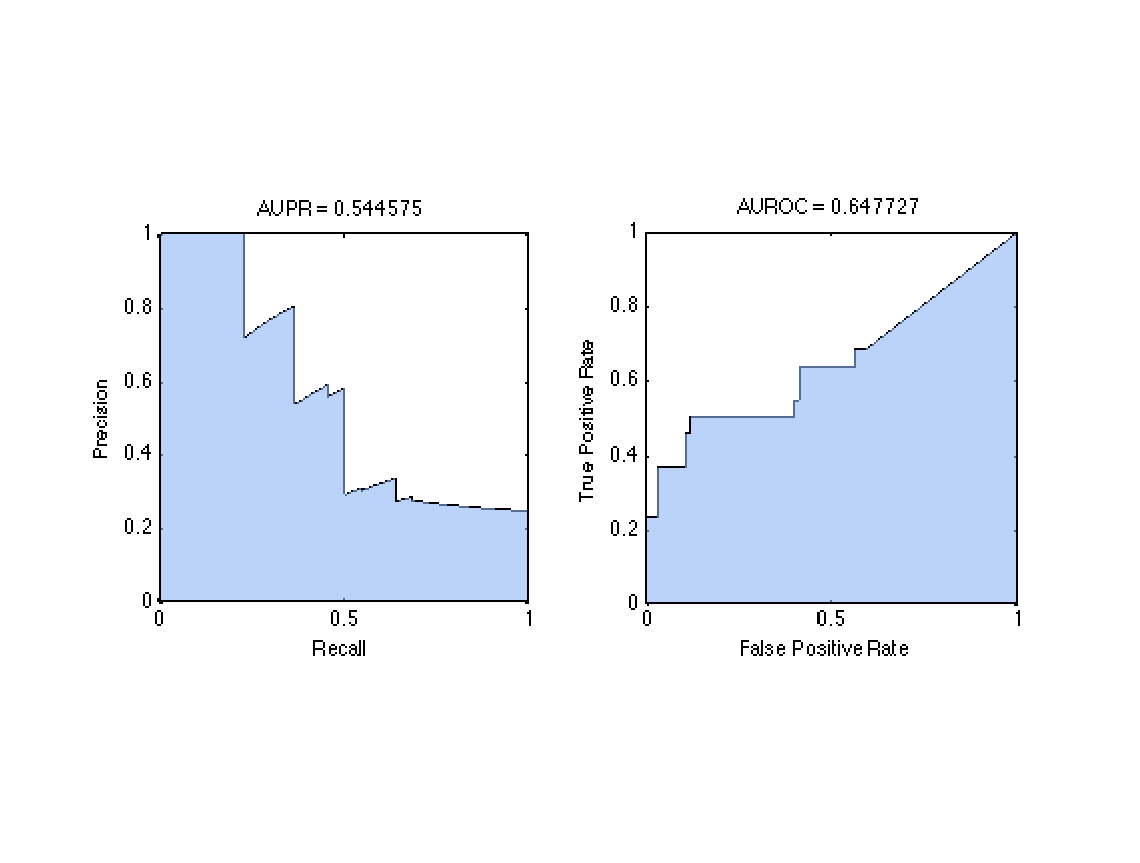
\includegraphics[width=\textwidth]{figures/PR-ROC}
\caption{\emph{Precision-Recall} (PR) and \emph{Receiver Operator Characteristic} (ROC) curves plotted with \emph{evaluation.m}. AUPR and AUROC (area under the curve) values are shown above the plots.}
\end{figure}


\vspace{\stretch{1}}

% ==================================================================================

\pagebreak
\small
\begin{thebibliography}{}

\addvspace{6pt}
\bibitem[Davis and Goadrich(2006)]{Davis2006}
Davis, J., and Goadrich, M. (2006) The Relationship Between Precision-Recall and ROC Curves. \emph{Proceedings of the 23rd international conference on Machine learning}, 233--240, 2006.\\

\bibitem[Marbach et~al.(2008)]{Marbach2008}
Marbach, D., Mattiussi, C., and Floreano, D. (2008) Combining Multiple Results of a Reverse Engineering Algorithm: Application to the DREAM Five Gene Network Challenge. \emph{Annals of the New York Academy of Sciences}. \emph{To appear}.\\

\bibitem[Marbach et~al.(2009)]{Marbach2009}
Marbach, D., Schaffter, T., Mattiussi, C., and Floreano, D. (2009) Generating Realistic \emph{in silico} Gene Networks for Performance Assessment of Reverse Engineering Methods. \emph{Journal of Computational Biology}. \emph{To appear}.\\

\end{thebibliography}

\end{document}
